\documentclass[11pt,spanish]{article}
\usepackage[utf8]{inputenc}
\usepackage{babel}
\usepackage{fullpage}
\usepackage{listings}
\usepackage{mathpazo}
\usepackage{enumitem}
\usepackage{courier}
\usepackage{xcolor}
\usepackage{textcomp}
\usepackage{amsmath}
\usepackage{amssymb}
\usepackage{tikz}
\usepackage{fancyhdr}
\usepackage{graphics}

\hyphenation{usua-rio usua-rios}

\newcommand{\titulo}{Certamen 2, sábado 14 de mayo de 2011}
\newcommand{\cc}[1]{\hfil\texttt{#1}\hfil}
\newcommand{\pond}[1]{[{\small\textbf{#1\%}}]}

\pagestyle{fancy}
\lhead{%
  {\Large\bfseries Programación---\titulo} \\
  Nombre: \nombre\hfill
  Rol:    \rol
  \vspace{2ex}
}
\chead{}\rhead{}\lfoot{}\cfoot{}\rfoot{}
\renewcommand{\headrulewidth}{0pt}
\addtolength{\headheight}{7ex}
\headsep=4ex


\newcommand{\onelinerule}{\rule[2.3ex]{0pt}{0pt}}
\newcommand{\twolinerule}{\rule[6.2ex]{0pt}{0pt}}
\newcommand{\respuesta}{\framebox[\textwidth]{\twolinerule}}
\newcommand{\nombre}{%
  \begin{tikzpicture}[xscale=.4,yscale=.7]
    \draw (0, 0) rectangle (22, 1);
  \end{tikzpicture}%
}
%\newcommand{\rol}   {\framebox[0.3\textwidth]{\onelinerule}}
\newcommand{\rol}{%
  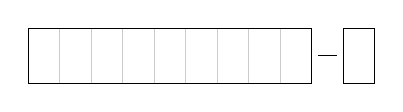
\begin{tikzpicture}[xscale=.4,yscale=.7]
    \draw[gray!40] ( 0, 0) grid      ( 9, 1);
    \draw          ( 0, 0) rectangle ( 9, 1);
    \draw          (10, 0) rectangle (11, 1);
    \draw (9 + .2, .5) -- (10 - .2, .5);
  \end{tikzpicture}%
}
\newcommand{\li}{\lstinline}
\providecommand{\pond}[1]{[{\small\textbf{#1\%}}]}

\lstdefinelanguage{py}{%
  classoffset=0,%
    morekeywords={%
      False,class,finally,is,return,None,continue,for,lambda,try,%
      True,def,from,nonlocal,while,and,del,global,not,with,print,%
      as,elif,if,or,yield,assert,else,import,pass,break,except,in,raise},%
    keywordstyle=\color{black!80}\bfseries,%
  classoffset=1,
    morekeywords={int,float,str,abs,len,raw_input,exit,range,min,max,%
      set,dict,tuple,list,bool,complex,round,sum,all,any,zip,map,filter,%
      sorted,reversed,dir,file,frozenset,open,%
      array,zeros,ones,arange,linspace,eye,diag,dot},
    keywordstyle=\color{black!50}\bfseries,%
  classoffset=0,%
  sensitive=true,%
  morecomment=[l]\#,%
  morestring=[b]',%
  morestring=[b]",%
  stringstyle=\em,%
}

\lstdefinelanguage{testcase}{%
  moredelim=[is][\bfseries]{`}{`},%
  backgroundcolor=\color{gray!20},%
}

\lstdefinelanguage{file}{%
  frame=single,%
}

\lstset{language=py}
\lstset{basicstyle=\ttfamily}
\lstset{columns=fixed}
\lstset{upquote=true}
\lstset{showstringspaces=false}
\lstset{rangeprefix=\#\ }
\lstset{includerangemarker=false}

\newlist{certamen}{enumerate}{1}
\setlist[certamen]{%
  label=\arabic*.,
  font=\LARGE\bfseries,%
  labelindent=-.5in,%
  leftmargin=0pt,%
  labelsep=1em%
}



\begin{document}

  \begin{enumerate}[font=\Large\bfseries]

    \item
      \pond{25}
      Indique qué es lo que imprimen los siguientes programas.

      \foreach \x in {1,2,...,8} {
        \noindent
        \begin{minipage}[b]{19.8em}
          \lstinputlisting{p\x.py}
          \framebox[18em]{\rule[6ex]{0pt}{0pt}}
          \vspace{0.7em}
        \end{minipage}
      }

    \newpage
    \item
      \pond{25}
      Las temperaturas mínimas y máximas
      de algunas ciudades de la región
      están guardadas en un diccionario
      cuyas llaves son las ciudades
      y cuyos valores son tuplas \texttt{(minima, maxima)}.

      Se desea generar un archivo
      cuyo contenido sea un reporte como el del ejemplo de más abajo.
      Los nombres de las ciudades en las que hubo más de 25 grados
      deben aparecer en mayúsculas.
      El nombre del archivo debe incluir la fecha.
      El orden en que aparecen las ciudades
      dentro del archivo no importa.

      Escriba la función \li!crear_reporte(fecha, temperaturas)!,
      cuyos parámetros son
      la fecha (una tupla \texttt{(año, mes, día)})
      y el diccionario de temperaturas,
      y que genere el archivo de texto
      con el formato del ejemplo.

      La función \li!crear_reporte! no debe retornar nada.
      Recuerde que \li!s.upper()!
      entrega el string \li!s! en mayúsculas.

      \begin{minipage}[T]{.45\textwidth}
        \lstinputlisting[linerange=CASO-]{pauta2.py}
      \end{minipage}
      \hfill
      \begin{minipage}[T]{.41\textwidth}
        Archivo \texttt{reporte-2011-5-14.txt}:
        \lstinputlisting[language=file]{reporte-2011-5-14.txt}
      \end{minipage}

    \newpage
    \item
      \pond{25}
      La red social Fookbace almacena la información de sus usuarios
      en un diccionario.
      Las llaves son un código numérico entero asignado a cada usuario, y
      los valores son tuplas con el nombre, la ciudad y la fecha de nacimiento del usuario.
      La fecha de nacimiento es una tupla \texttt{(año, mes, día)}:
      \lstinputlisting[linerange=USUARIOS-FIN\ USUARIOS]{pauta3-4.py}
      \begin{enumerate}
        \item Escriba la función \li!misma_ciudad(u1, u2)!,
          que indique si los usuarios con códigos \li!u1! y \li!u2!
          viven en la misma ciudad.
          \lstinputlisting[linerange=CASO\ MISMA\ CIUDAD-FIN\ CASO\ MISMA\ CIUDAD]{pauta3-4.py}
        \item Escriba la función \li!diferencia_edad(u1, u2)!,
          que retorne la diferencia de edad entre los usuarios
          cuyos códigos son \li!u1! y \li!u2!.
          (Utilice sólo el año de nacimiento de los usuarios
          para calcular la diferencia, no el mes ni el día).
          \lstinputlisting[linerange=CASO\ DIFERENCIA\ EDAD-FIN\ CASO\ DIFERENCIA\ EDAD]{pauta3-4.py}
      \end{enumerate}

    \newpage
    \item
      \pond{25}
      (Este ejercicio es una continuación del anterior).

      Para guardar la información sobre cuáles de sus usuarios son amigos entre sí,
      Fookbace utiliza el conjunto \li!amistades!,
      que contiene tuplas con los códigos de dos usuarios.
      Si la tupla \li!(a, b)! está dentro del conjunto,
      significa que los usuarios con códigos \li!a! y \li!b! son amigos.
      En todas las tuplas se cumple que \(\text{\li!a!} < \text{\li!b!}\).
      \lstinputlisting[linerange=AMIGOS-FIN\ AMIGOS]{pauta3-4.py}
      \begin{enumerate}
        \item Escriba la función \li!obtener_amigos(u)!,
          que retorne el conjunto de los códigos
          de los amigos de \li!u!.
        \item Escriba la función \li!recomendar_amigos(u)!,
          que retorne el conjunto de los códigos
          de los usuarios que cumplen todas estas condiciones a la vez:
          \begin{itemize}
            \item son amigos de un amigo de \li!u!,
            \item no son amigos de \li!u!,
            \item viven en la misma ciudad que \li!u!, y
            \item tienen menos de diez años de diferencia con \li!u!.
          \end{itemize}
      \end{enumerate}
      En ambas funciones,
      el parámetro \li!u! es el código de un usuario,
      y el valor de retorno es un conjunto de códigos de usuarios.
      Recuerde que \li!c.add(x)! agrega el valor \li!x! al conjunto \li!c!.

  \end{enumerate}
\end{document}

